\documentclass{article}

% Language setting
% Replace `english' with e.g. `spanish' to change the document language
\usepackage[spanish]{babel}
\usepackage{fancyhdr}
\usepackage{graphicx}

% Set page size and margins
% Replace `letterpaper' with `a4paper' for UK/EU standard size
\usepackage[letterpaper,top=2cm,bottom=2cm,left=3cm,right=3cm,marginparwidth=1.75cm]{geometry}

\pagestyle{fancy}
\fancyhead{}\fancyfoot{}
\fancyhead[L]{
    
\includegraphics[width=3.5cm]{ucentral1.png}
} 
\fancyhead[C]{\thepage}
\fancyhead[R]{
    
\includegraphics[width=2cm]{r.png}
}

\fancyfoot[L]{}
\fancyfoot[C]{\thepage}
\fancyfoot[R]{}

\renewcommand{\footrulewidth}{0.5pt}
\setlength{\headheight}{60pt} % ajusta la altura del encabezado y pie de página
\renewcommand{\headrulewidth}{0.5pt}

% Useful packages
\usepackage{amsmath}
\usepackage{graphicx}
\usepackage[colorlinks=true, allcolors=blue]{hyperref}

\title{Fundamentos de estadistica para analitica de datos} 

\author{Juan Salazar - Camilo Alarcon}

\begin{document}
\maketitle
\thispagestyle{fancy}

\begin{abstract}

El presente trabajo de estadísticas se enfoca en el análisis de los resultados de las pruebas ICFES en Colombia(Bogota) en los últimos años. A través de diversas técnicas estadísticas, se pretende examinar los datos y extraer conclusiones relevantes sobre el desempeño de los estudiantes en diferentes áreas de conocimiento, identificar patrones y tendencias, y explorar los factores que pueden influir en los resultados de las pruebas. \hfill \break

\end{abstract}

\section{Introduction}

Las pruebas ICFES son un instrumento de evaluación que se utiliza en Colombia para medir el conocimiento y las habilidades de los estudiantes de educación secundaria y para evaluar su capacidad para ingresar a la educación superior. Desde su creación en 1967, estas pruebas han sido objeto de diversos estudios y análisis estadísticos que han permitido conocer mejor los resultados obtenidos por los estudiantes, así como identificar fortalezas y debilidades del sistema educativo en Colombia. \hfill \break

El presente trabajo de estadísticas tiene como objetivo principal analizar los resultados de las pruebas ICFES en Colombia en los últimos años, con el fin de identificar tendencias, patrones y posibles factores que puedan influir en el rendimiento de los estudiantes. Para ello, se aplicarán diversas técnicas estadísticas que permitirán examinar los datos y extraer conclusiones relevantes sobre el desempeño de los estudiantes en diferentes áreas de conocimiento. \hfill \break

Es importante destacar que el análisis de los resultados de las pruebas ICFES puede ofrecer información valiosa para la toma de decisiones en el ámbito educativo. A través de la identificación de las fortalezas y debilidades del sistema educativo, se pueden implementar estrategias que permitan mejorar la calidad de la educación en Colombia y, por ende, la formación de los estudiantes. \hfill \break

En resumen, el presente trabajo de estadísticas se enfoca en analizar los resultados de las pruebas ICFES en Colombia, con el objetivo de ofrecer información útil que permita mejorar la educación en el país. A través del análisis estadístico de los datos, se espera identificar las áreas de mejora y proponer soluciones que contribuyan a la formación de estudiantes más preparados y competitivos.\hfill \break
\newline
\newline
\newline
\newline
\newline
\newline
\newline
\newline
\newline


\section{Aplicaciones utilizadas}

\subsection{Control de versiones}

\hfill \break
\newline
\begin{center}
\begin{tabular}{ c c  }

\includegraphics[scale=0.3]{git.png} & \href{https://github.com/Juan-Salazar-Saenz/R/tree/master/Tarea_1}{
\includegraphics[scale=0.3]{github.png}} 
\end{tabular}
\end{center}

\subsection{hernel + entorno}

\hfill \break
\newline
\begin{center}
\begin{tabular}{c c c}

\includegraphics[scale=0.1]{r.png} & 

\includegraphics[scale=0.1]{vscode.png}  & 

\includegraphics[scale=0.2]{platzi.png} \\
\end{tabular}
\end{center}
\newpage

\subsection{Limpieza de entorno y cargue de la base para analisis}

\begin{center}
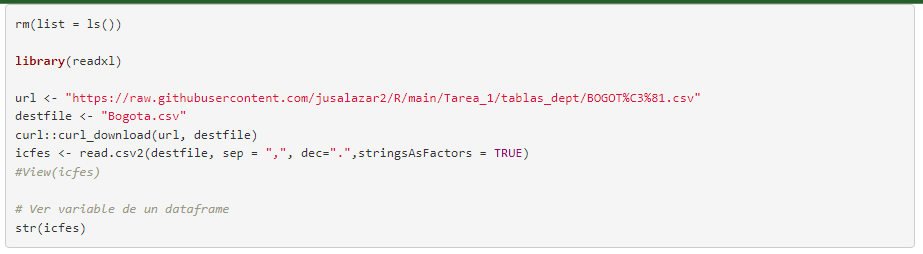
\includegraphics[scale=0.5]{Captura.PNG} 
\end{center}

\subsection{Describimos nuestra base para entender que tenemos y como podemos comenzar el analisis}

\begin{center}
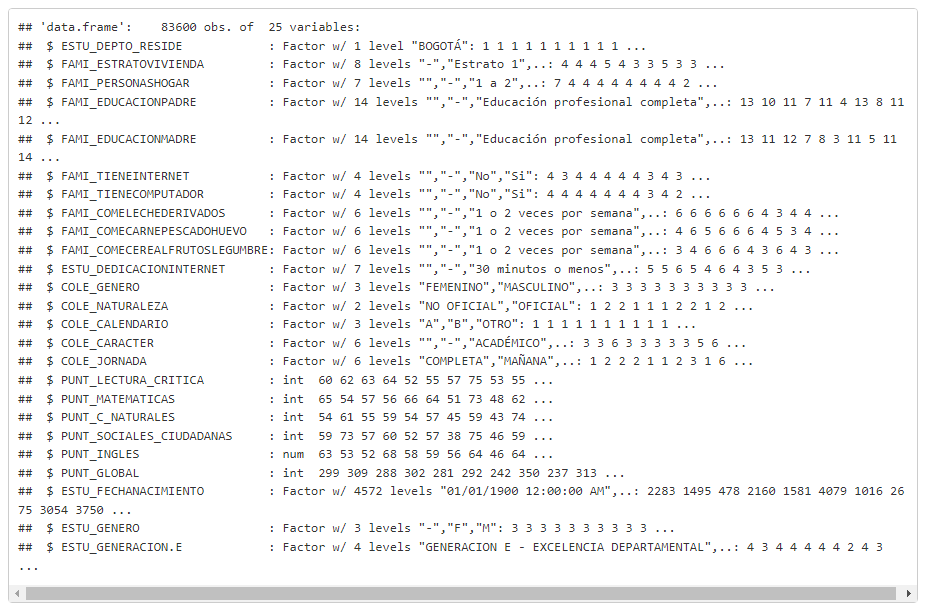
\includegraphics[scale=0.5]{Captura1.PNG} 
\end{center}


\begin{center}
\subsection{Validamos el nombre de los campos para comenzar a trabajar con ellos}


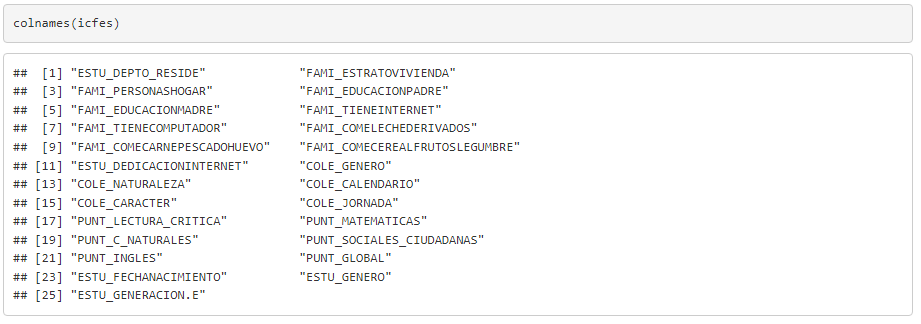
\includegraphics[scale=0.5]{Captura2.PNG} 
\end{center}
\newpage

\subsection{Mejor puntuacion por genero}

seleccionamos la data

\begin{center}
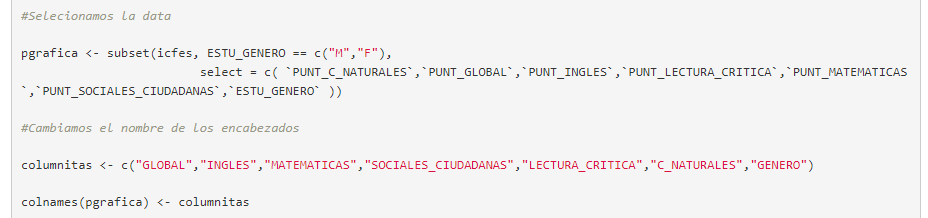
\includegraphics[scale=0.5]{Captura3.PNG} 
\end{center}

graficamos el resultado

\begin{center}
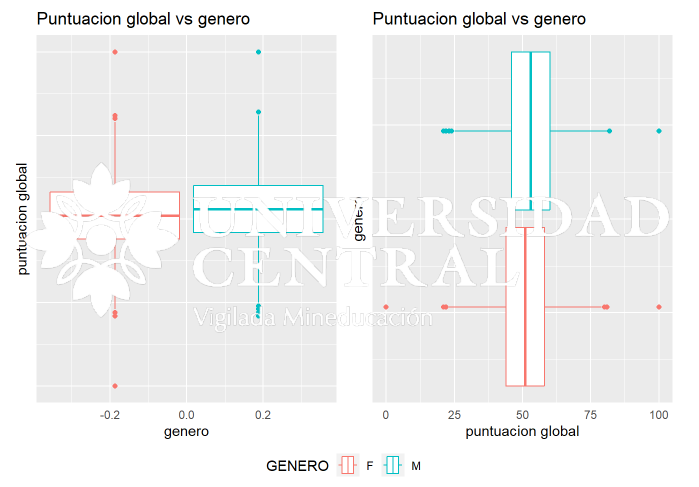
\includegraphics[scale=0.5]{Captura4.PNG} 
\end{center}
\newpage

\subsection{Generamos una grafica de punto para ver la distribucion de los participantes de la presentacion del examen}

\begin{center}
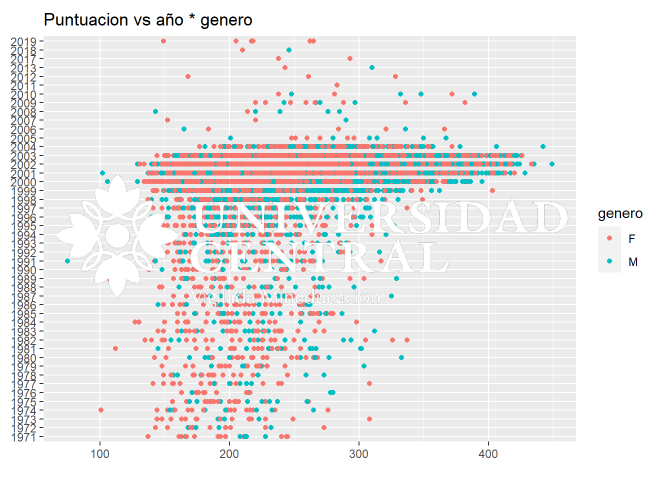
\includegraphics[scale=0.6]{Captura5.PNG} 
\end{center}

Si hacemos un poco de zoom para ver el mejor resultado de todos, podemos observar que en el año 2002 una mujer lo obtuvo

\begin{center}
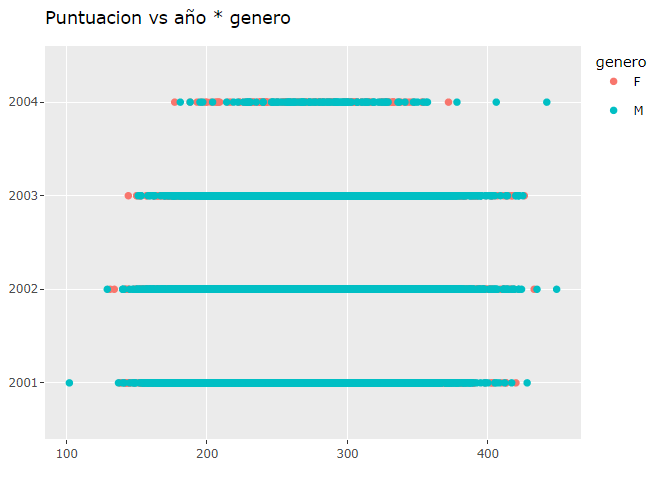
\includegraphics[scale=0.5]{Captura6.PNG} 
\end{center}

\subsection{Verificaremos que grupo obtuvieron el mejor puntaje}

\begin{center}
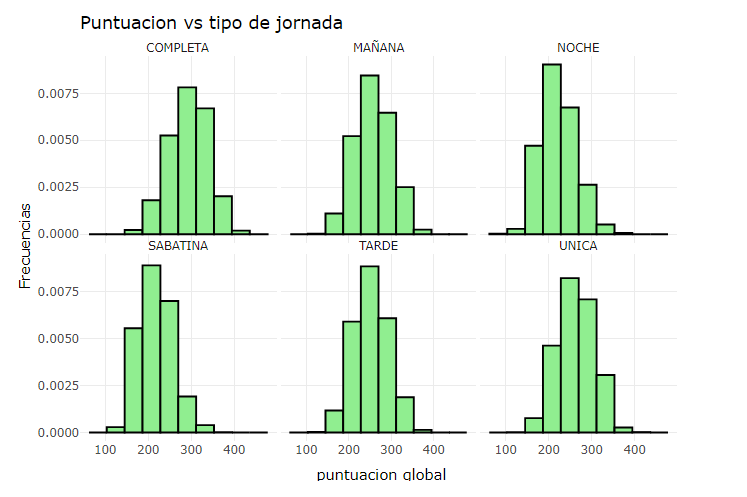
\includegraphics[scale=0.5]{Captura7.PNG} 
\end{center}

\subsection{Validaremos el estrato con mas participantes}

\begin{center}
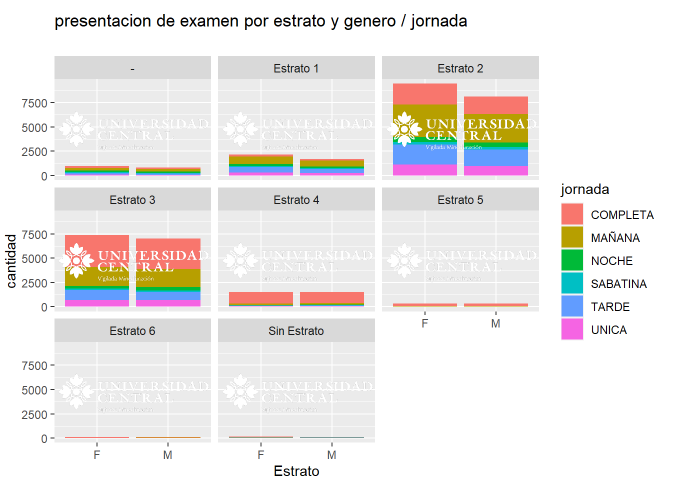
\includegraphics[scale=0.5]{Captura8.PNG} 
\end{center}

\subsection{Validaremos el acceso a internet de los participantes}

\begin{center}
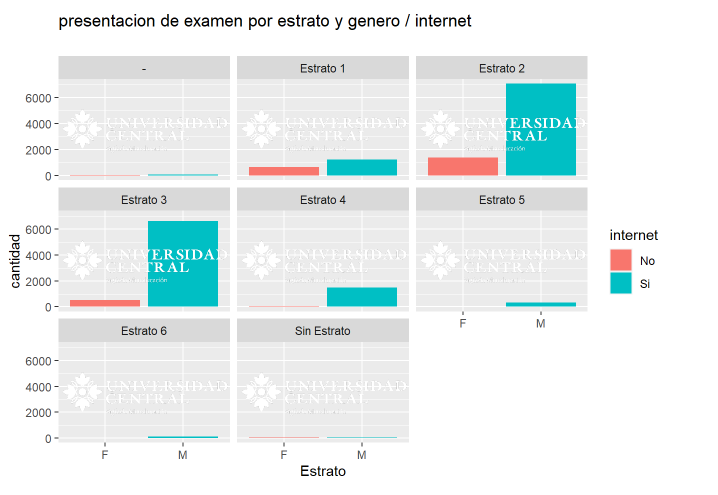
\includegraphics[scale=0.5]{Captura9.PNG} 
\end{center}

\subsection{Validaremos la distribucion de los participantes por año de nacimiento}

\begin{center}
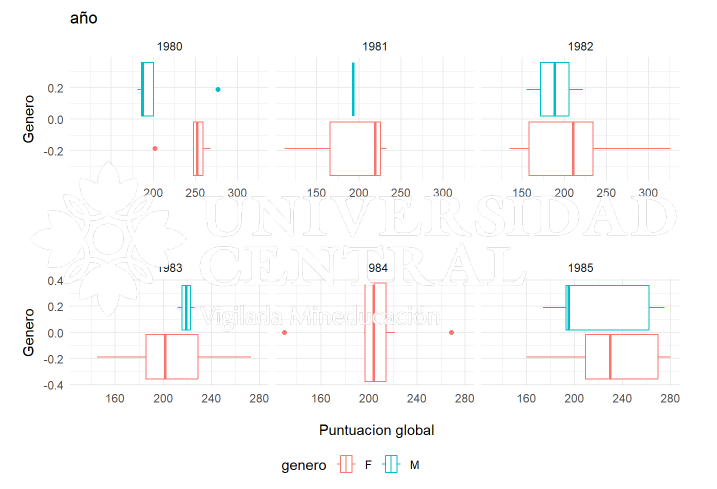
\includegraphics[scale=0.5]{Captura10.PNG} 
\end{center}
\begin{center}
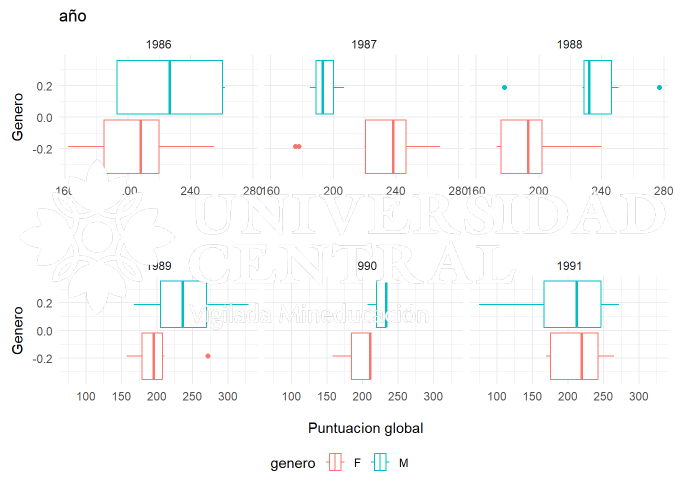
\includegraphics[scale=0.5]{Captura11.PNG} 
\end{center}
\begin{center}
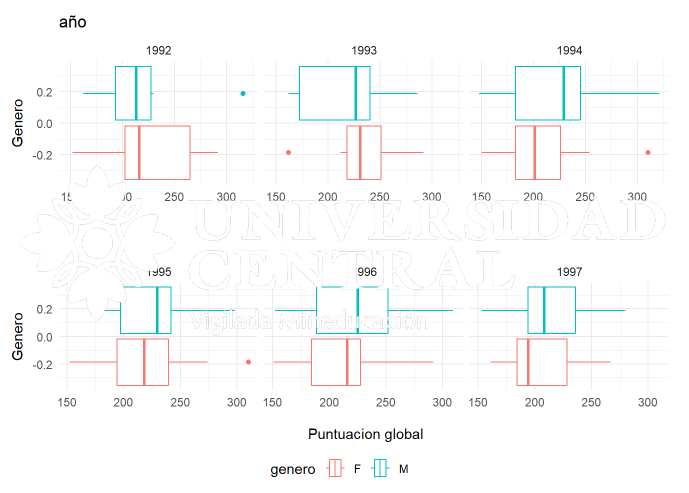
\includegraphics[scale=0.5]{Captura12.PNG} 
\end{center}
\begin{center}
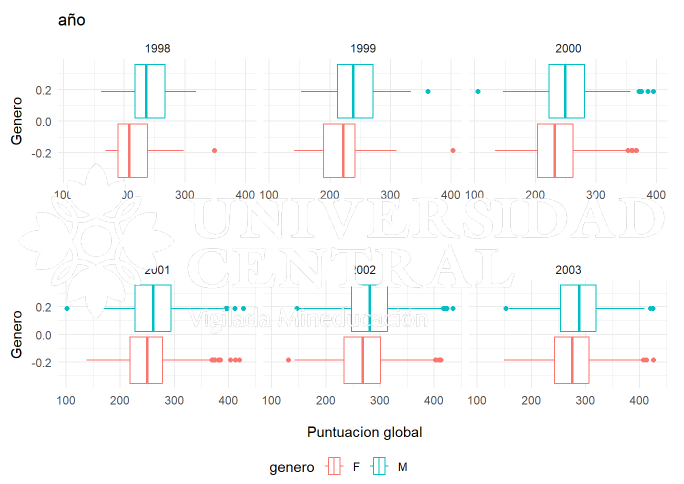
\includegraphics[scale=0.5]{Captura13.PNG} 
\end{center}
\begin{center}
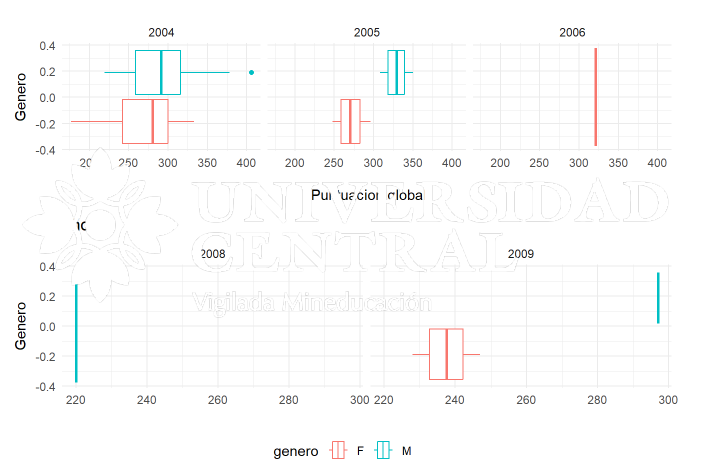
\includegraphics[scale=0.5]{Captura14.PNG} 
\end{center}
\begin{center}
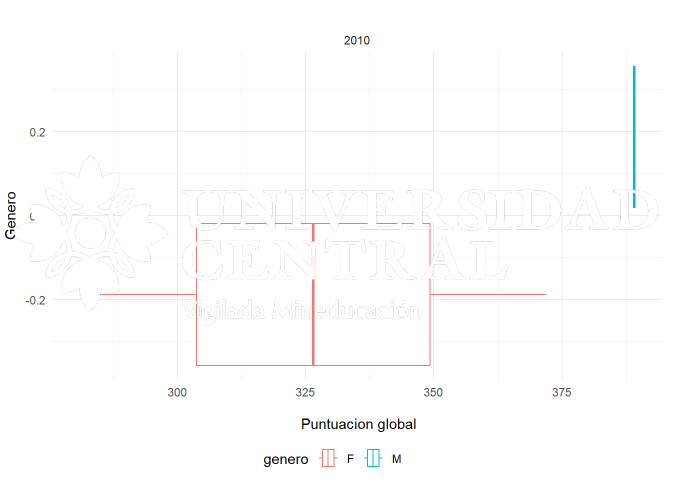
\includegraphics[scale=0.5]{Captura15.PNG} 
\end{center}
\begin{center}
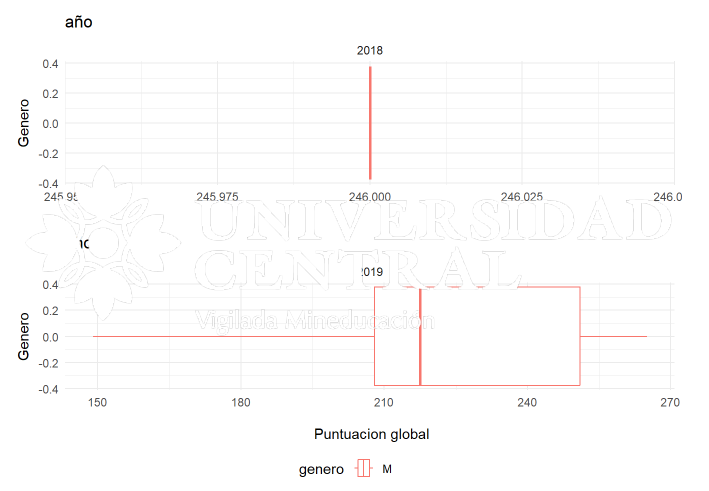
\includegraphics[scale=0.5]{Captura16.PNG} 
\end{center}

\subsection{Validaremos el nucleo familiar vs estrato / con acceso a internet de los participantes}

\begin{center}
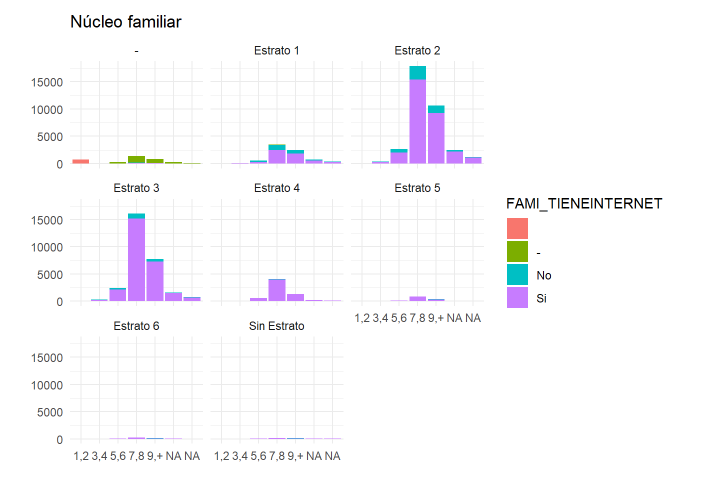
\includegraphics[scale=0.5]{Captura17.PNG} 
\end{center}

\subsection{Educacion de los padres}

\begin{center}
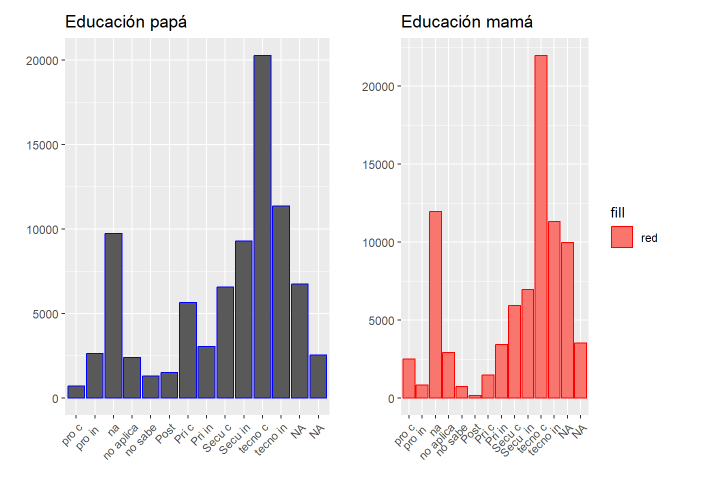
\includegraphics[scale=0.5]{Captura18.PNG} 
\end{center}

\subsection{Graficaremos la densidad de las pruebas para medir el mejor resultado}

\begin{center}
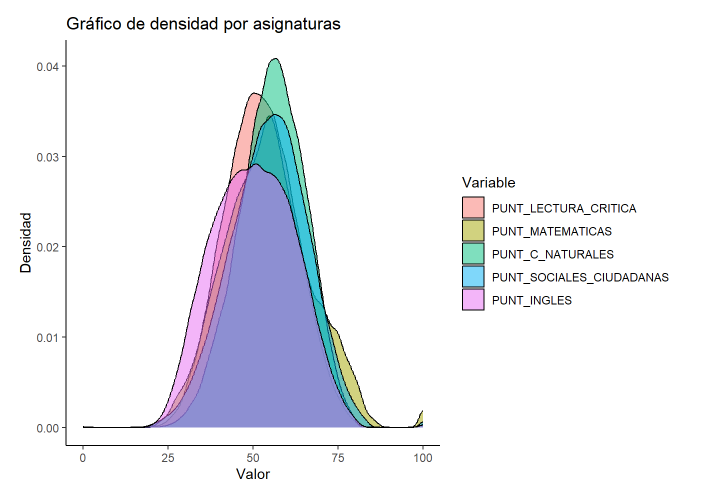
\includegraphics[scale=0.5]{Captura19.PNG} 
\end{center}

\subsection{Graficamos la relacion del punto global con distintos factores}

\begin{center}
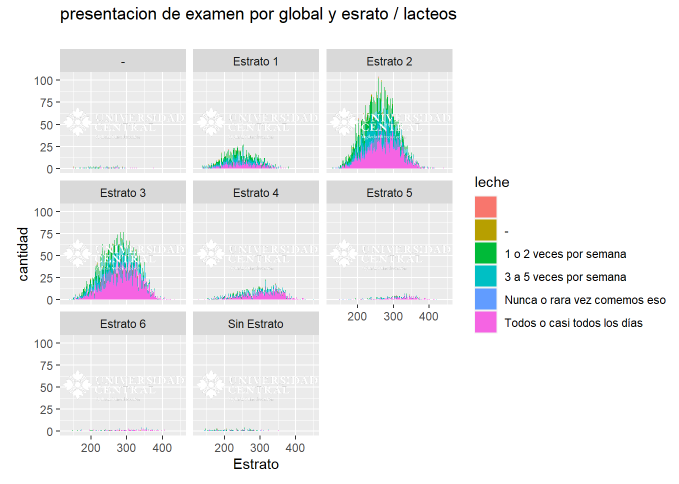
\includegraphics[scale=0.6]{Captura20.PNG} 
\end{center}
\begin{center}
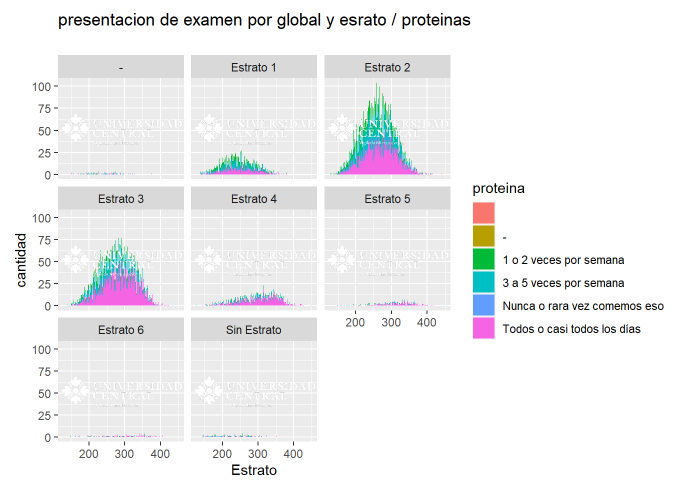
\includegraphics[scale=0.6]{Captura21.PNG} 
\end{center}
\begin{center}
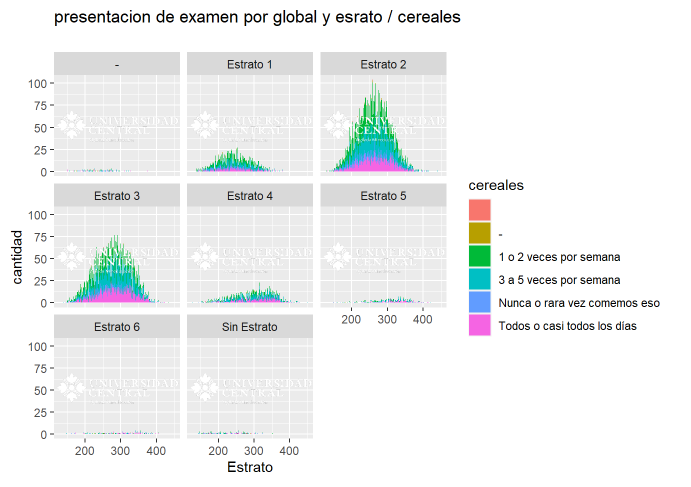
\includegraphics[scale=0.6]{Captura22.PNG} 
\end{center}
\begin{center}
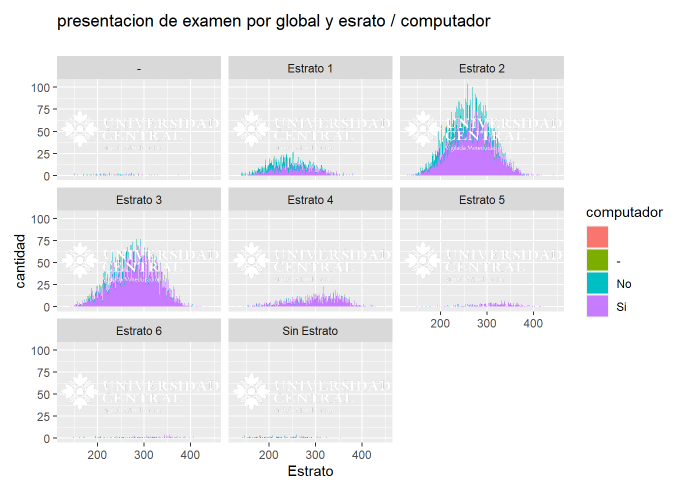
\includegraphics[scale=0.6]{Captura23.PNG} 
\end{center}

\section{Conclusiones}

\subsection{La base de bogota esta rara}

Despues de ver las distribuciones de las graficas pordemos concluir que, los estratos que mas participan de este examen son el 2 y 3, en su mayoria mujeres, pero mucha de la poblacion tiene acceso al internet, pero sin duda las personas que mas le meten ganas son las de jornada norturna

\bibliographystyle{alpha}
\bibliography{sample}

\end{document}